\bookchapter{Capítulo 37: La revolución de paradigma — de «escribir código» a «dirigir a la IA que escribe código»}

\chapterintro{Enhorabuena: si estás leyendo este libro, estás en pleno centro de una revolución de paradigma profesional. El punto de partida fue una frase que un programador publicó en redes sociales en 2025. ¿Te suena dramático? Pues así ocurrió.}

\booksection{El nacimiento del Vibe Coding: un movimiento provocado por una frase}

En febrero de 2025, Andrej Karpathy —recuerda este nombre, lo volverás a ver varias veces— publicó en redes sociales un tuit que después se citaría una y otra vez: «Hay una nueva forma de programar que se llama Vibe Coding: te dejas llevar totalmente por las sensaciones (vibes), ignoras los detalles del código y dejas que la IA lo haga todo. Dices lo que ves, copias y pegas, y con que funcione a grandes rasgos basta».

Ese comentario, que parecía dicho al pasar, bautizó con precisión un cambio de paradigma que ya se estaba produciendo en silencio: el ser humano deja de escribir código línea a línea y pasa a describir su intención en lenguaje natural, y la IA se encarga de la implementación. El tono de Karpathy tenía un punto de burla, pero escondía una idea profunda: cuando la capacidad de generar código de la IA cruza cierto umbral, el cuello de botella de la programación ya no es «¿soy capaz de escribir esta línea?», sino «¿tengo claro lo que quiero hacer?».

\begin{tcbinfo}{Consejo: ¿qué es un vibe?}
Vibe se traduce literalmente como «ambiente, sensación». Vibe Coding es «dirigir la programación de la IA siguiendo tu sensación»: tú describes lo que quieres y la IA se encarga de implementarlo. Recuerda esta palabra: es el «acta de nacimiento» de esta revolución.

\end{tcbinfo}

Desde ese momento, el significado de «programar» se escindió: la programación tradicional traduce un diseño a sintaxis; la nueva traduce una intención en instrucciones. La primera pone a prueba los dedos; la segunda, el cerebro.

El término Vibe Coding pasó pronto de la broma al concepto serio de ingeniería. A mediados de 2026 ya había evolucionado de meme de redes sociales a un sistema metodológico completo que cubre todo el proceso: la expresión de requisitos, la gestión del contexto, la verificación iterativa y la garantía de calidad. También se tomó conciencia de que «ir a sensaciones» es solo el estado de la fase de iniciación: la programación con IA realmente eficaz exige una forma de pensar sistematizada. Y esa forma de pensar es justo lo que este libro quiere darte.

\booksection{El panorama en 2026: la era del Agentic Engineering}

Para agosto de 2026, el campo de la programación con IA ya había atravesado varias iteraciones de paradigma importantes. El Vibe Coding fue la chispa inicial, pero pronto se vio que, si solo «ibas a sensaciones» charlando con la IA, la calidad del código resultante era muy inestable: a veces brillante, a veces un desastre. Así que el paradigma empezó a evolucionar: de la simple programación conversacional a la ingeniería de agentes estructurada.

De nuevo Karpathy: a comienzos de 2026 propuso el concepto de Agentic Engineering. A diferencia del «lo pides y lo genera» del Vibe Coding, el Agentic Engineering enfatiza darle a la IA un objetivo para que planifique por sí sola los pasos, use herramientas, verifique los resultados y corrija iterando. La IA deja de ser un simple generador de código y pasa a ser un agente (Agent) capaz de percibir su entorno, tomar decisiones y ejecutar acciones.

Este giro trajo tres cambios clave:

\begin{enumerate}
  \item Cambia el modo de interacción: del «pregunta y respuesta» a «fijar el objetivo y delegar».
  \item Cambia el producto del trabajo: de «un fragmento de código» a «un proyecto completo».
  \item Cambia el papel de la persona: de «revisar el código línea por línea» a «definir los límites y aceptar los resultados».
\end{enumerate}

Los números no mienten: en Cursor 3, publicado en abril de 2026, el uso del modo Agent superó por primera vez al del autocompletado con Tab, señal de que los desarrolladores ya habían migrado en masa a esta forma de trabajar; y Claude Code, la herramienta de programación con IA nativa de terminal, alcanzó a mediados de 2026 unos ingresos anualizados de 2.500 millones de dólares. Este gráfico de tendencias te permite intuir ese momento del cruce:

\begin{center}
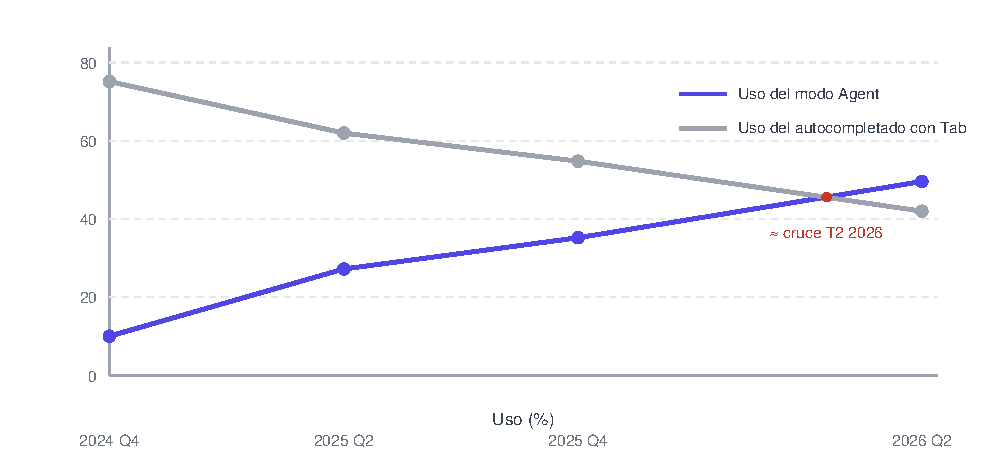
\includegraphics[width=0.92\linewidth]{figures/fig-di-san-shi-qi-zhang-1}
\\[2pt]\small Figura 1: tendencia de uso de los modos de interacción de la programación con IA (estimación a partir de datos de estudios del sector; en el segundo trimestre de 2026 el modo Agent supera al autocompletado con Tab)
\end{center}

Pero seamos sinceros: los cambios de herramientas y de modelos son solo la superficie. Uses Cursor o Claude Code, y sea GPT-5 o Claude 4.5 el modelo de fondo, quienes triunfan programando con IA siguen todos la misma metodología de base. Eso es lo que esta guía quiere enseñarte.

\booksection{El cambio mental clave: de Coder a Conductor}

La formación tradicional en programación te enseña a ser un Coder: entender la sintaxis, memorizar API, depurar errores lógicos. En la era de la programación con IA, ese rol se está redefiniendo. Ya no necesitas escribir cada línea con tus propias manos, pero sí convertirte en un «director» (Conductor): definir el campo de batalla, fijar las reglas, repartir las tareas y aceptar los resultados.

La esencia de este giro no está en «¿sabes programar?», sino en «¿sabes pensar con claridad qué quieres hacer?». Un gran director no tiene por qué ser el mejor soldado, pero debe conocer mejor que nadie el objetivo de la campaña, el terreno y el despliegue de las tropas. Igualmente, quien programa bien con IA no tiene por qué dominar los detalles de sintaxis de cada lenguaje, pero debe tener clarísimos el objetivo del proyecto, las restricciones de arquitectura y los estándares de calidad.

Merece la pena mirar esta tabla dos veces: resume todo lo que implica este cambio de rol:

\begin{center}
\begin{tabularx}{\linewidth}{|X|X|X|}
\hline
\textbf{Dimensión} & \textbf{Coder tradicional} & \textbf{Director con IA (Conductor)} \tabularnewline
\hline
Habilidad central & Memorizar sintaxis, llamar API, depurar & Definir requisitos, gestionar el contexto, juzgar los resultados \tabularnewline
Modo de trabajo & Escribir el código línea a línea & Describir la intención y revisar la producción \tabularnewline
Control de calidad & Lo escribí yo y sé dónde puede fallar & Validar la producción de la IA con pruebas y revisiones \tabularnewline
Conocimientos requeridos & Dominio profundo de un lenguaje/framework concreto & Comprensión amplia del panorama técnico y profunda de la lógica de negocio \tabularnewline
Dónde está el cuello de botella & La velocidad de codificación y la memoria de sintaxis & La claridad de pensamiento y la capacidad de expresión \tabularnewline
Origen de los errores & Errores de sintaxis, omisiones lógicas & Requisitos vagos, contexto insuficiente \tabularnewline
\hline
\end{tabularx}
\end{center}

\begin{center}\small\color{gray}Comparación por dimensiones entre el Coder tradicional y el director con IA\end{center}

Esto no significa, ni de lejos, que el conocimiento de programación ya no importe. Al contrario: solo cuando entiendes el código que escribe la IA puedes revisarla y corregirla con eficacia; solo cuando comprendes estructuras de datos y algoritmos puedes juzgar si la propuesta de la IA es razonable. Tus conocimientos marcan tu «techo de mando», pero su papel pasa de «herramienta de ejecución» a «base para juzgar».

\booksection{Por qué la metodología importa más que las herramientas}

Las herramientas se renuevan cada tres meses; la metodología evoluciona cada tres años. Lo que aprendas a hacer con una herramienta puede quedarse obsoleto en tres meses; un modo de pensar bien asentado seguirá siendo válido dentro de tres años.

Mucha gente, al empezar con la programación con IA, lo primero que pregunta es «¿cuál es la mejor herramienta?» o «¿cuál es el modelo más potente?». No son preguntas irrelevantes, pero se preguntan en el orden equivocado. El panorama de herramientas de agosto de 2026 ya no se parece en nada al de agosto de 2025: Trae, Qoder y otras herramientas han subido y bajado, Cursor pasó de extensión a IDE independiente y luego evolucionó a Cursor 3, y Claude Code pasó de proyecto experimental a opción dominante para programar en la terminal. Pero detrás de ese volcán de cambios, los principios de pensamiento de quienes triunfan casi no han variado.

Por eso este libro no gasta páginas en enseñarte las operaciones concretas de una herramienta: eso queda obsoleto nada más escribirse. En cambio, todo su peso está en una metodología de pensamiento contrastada: cómo pensar los requisitos, cómo comunicarte con la IA, cómo validar la producción, cómo iterar sin parar. Si dominas esa metodología, te adaptarás rápido a cualquier herramienta; si solo aprendes los botones, cada herramienta nueva será empezar de cero.

\begin{tcbinfo}{Para los lectores que parten de cero: respira tranquilo}
Si partes de cero, no te asuste la palabra «metodología». No es una filosofía abstracta: es un manual operativo de «cómo pensar cuando te surge un problema». Es como aprender a cocinar: puedes seguir la receta paso a paso (operar las herramientas), pero el buen chef entiende por qué se sazona así y cómo se controla el fuego (la metodología). Este libro arranca desde los conceptos más básicos y cada principio viene acompañado de casos comparativos concretos, para que no solo entiendas el «qué es», sino que domines el «cómo se hace».

\end{tcbinfo}

\begin{tcbpractice}{Manos a la obra: hazte una «foto de rol» de tu yo actual}
Coge un papel y escribe las respuestas a tres preguntas: (1) ¿Cómo usas ahora la IA para ayudarte a programar (si lo has hecho)? (2) ¿Te pareces más al «Coder» o al «director» de la tabla de arriba? (3) ¿Cómo te gustaría que el tú de dentro de tres meses describiera su forma de trabajar? Guarda el papel dentro del libro y vuelve a leerlo al terminar el capítulo 47: verás que el cambio va más rápido de lo que imaginas.

\end{tcbpractice}

\begin{tcbsummary}{Resumen del capítulo}
\begin{itemize}
  \item En 2025, Karpathy bautizó con «Vibe Coding» la revolución de la programación con IA: de escribir código línea a línea a describir la intención en lenguaje natural
  \item En 2026 se evolucionó al Agentic Engineering: se da el objetivo, se delega, la IA planifica y ejecuta sola, y la persona se reserva la aceptación
  \item En Cursor 3, el modo Agent superó por primera vez al autocompletado con Tab; Claude Code alcanzó 2.500 millones de dólares de ingresos anualizados
  \item Tu nuevo rol es el de Conductor (director): definir el campo de batalla, fijar las reglas, repartir las tareas y aceptar los resultados
  \item Las herramientas se renuevan cada tres meses; la metodología evoluciona cada tres años: aprende metodología, no operaciones
\end{itemize}

\end{tcbsummary}
